\documentclass[12pt]{article}

\usepackage{graphicx}

\usepackage{setspace}
\setstretch{1.25}

\begin{document}  
  \begin{titlepage}
\begin{center}
\huge{\bfseries{Project Report:}}\\
[2mm]
\huge{\bfseries{Dental Clinic Management System}}\\
Version 2.0 : Laboratory Exercise-03\\
  \vskip 0.2in
  \large{\bfseries{Front-End Development:}}\\
 Prince Ngema (754774)\\
 Luyanda Makhoba (834867) \\
 
 \large{\bfseries{Back-End Development:}}\\
 Takatso Molekane (569869)\\
 Tholithemba Mngomezulu (1512124)\\
 
\end{center}
 \end{titlepage}
 \tableofcontents
 \newpage
\section{Introduction}

\subsection{Purpose}
This document serves to describe the processes undertaken in the inception of the Dental Clinic Management system software prototype. The purpose of this document is to provide a detailed description of the DCMS ,a web application.It will give in detail the purpose of the system, features of the system  and the constraints under which the system will operate.
\subsection{Problem Statement}
Managing a dental clinic may be cumbersome at times, the paperwork that the receptionist have to do and the time  patients have to spend waiting in queue is excessive.Hard copy files stored in cabinets pose a security threat since it is possible for unauthorized personel to gain access because of negligence.Human error in the collection and capturing of data occurs when patients either fill in their details incorrectly or the receptionist captures the data wrongly.Paper files are hard to back up. 
\subsection{Project Objectives }
The software is aimed at replacing manual paper systems that currently exists at a dental clinic.Users will remotely have access to relevant services based on requirements.The project objectives are :
\begin{itemize}
\item reduce the paper work the receptionist have to do on daily basis
\item cut the amount of waiting time in queues
\item ensure and protect patient's privacy
\item reduce human error in capturing data
\item reduce paper work for doctors
\end{itemize}
\subsection{Stakeholders}
Anyone that is influenced by or influences a project is a stakeholder. There are two types of stakeholders , internal and external stakeholders.
\begin{itemize}
\item \textbf{External}
\begin{itemize}
\item Patients\\
Patients are able to make appointments and view their bill 
\item Dentist\\
Dentists can login ,view and set their own schedule of appointments. Write      out a prescription for a patient and view a patient's profile(medical record).
\item Receptionist\\
receptionist logs in with their username and password, views and manages  appointments, performs day open and close activities. He also sends reports to admin and help with registering those patients who that are having problems with registering.
\item Admin \\
The administrator has the authority to add or remove a doctors and receptionist.He grants permission to receptionist  and  dentists the authority to view and generates report.He also has the authority to add or delete patients from system. He also manages the system
\end{itemize}
\item \textbf{Internal}
\begin{itemize}
\item  Scrum team \\
responsible for developing the software
\item Product owner\\
someone in charge of the entire project
\item Scrum master \\
 The link between the scrum team and the product owner(project manager)
\item Equipment suppliers \\
They supply the hardware needed for the operation of the system.(i.e) Computers
\end{itemize}
\end{itemize}
\subsection{Scope}
Define what the following sections do

\subsection{Definitions,Acronyms and Abbreviations}
\begin{tabular}{|p{3cm}|p{9cm}|}
\hline
\textbf{Term} & \textbf{Definition}\\
\hline
DCMS &  A Dental Clinic Management System application\\
\hline
User &  Anyone who will be interacting directly with the system..\\
\hline
Netbeans & an integrated development environment for java\\
\hline
Java & A general-purpose computer-programming language that is concurrent, class-based,object-oriented\\
\hline
PHP & Hypertext Preprocessor is a server-side scripting language designed for web development. \\
\hline
Json & JavaScript Object Notation is an open-standard file format that uses human readable text to transmit data objects consisting of attribute-value pairs and array data types \\
\hline
\end{tabular}

\subsection{References}
\begin{itemize}
    \item    
    IEEE Recommended Practice for Software Requirements Specifications
    \item
    https://www.bmc.com/blogs/software-requirements-specification-how-to-write-srs-with-examples/ (Accessed Aug 2018)
    \item
    Zainab Murtadha- Dentist Web Based Patient Information System and Services in Cloud
    \item
    Virtual Medical Home SRS-Bapuju Institute
    \item
    https://krazytech.com/projects
    \end{itemize}
    \newpage

54\subsection{Project Overview}
\textbf{Front End tasks:}
    This involves the making of User Interfaces. These are the screens that the users will be seeing when using the system.
    \begin{itemize}
    \item
    Create Patient(Input will be patient details)
    \item
    Log in(Username and Password)
    \item
    Create Appointment(PatientId and Date/Time)
    \item
    Create Bill(PatientID, DoctorID and Consultation Details)
    \item
    View Schedule(DoctorID and Date/Time)
    \item
    View Bill(PatientID)
    \end{itemize}
    \textbf{Back End tasks:}
    \begin{itemize}
    \item
    Create Database with table and entities as listed in ERD
    \item
    Use back-end frameworks to build server-side software. PHP and JSON    
    \item
    Cloud computing integration-Allowing Database to be accessed remotely.
    \end{itemize}

\subsubsection{Existing System}
The present system is manual based. It involves paper work in the form of mantaining files, making appointments and billing.The manually based system has the following disadvantages:
\begin{itemize}
\item
it is a limited system.
\item
looking for a patient's file may take a long time
\item
patients have to queue to make an appointment
\item
There is no backup files.
\item
files are prone to damage.
\item
editing file problems.
storage space may be limited.
\item
Patient's personal information is not protected, it can be accessed by anyone.
\end{itemize}


\section{Software Requirements Specifications}
\subsection{Overall Description}t
\subsubsection{Product perspective}

\subsection{Functionality}
\subsection{Usability}
\newpage   
\section{Project Design and Architecture}
 
    \subsubsection{Architecture}
    
    \begin{figure}[h]
    \centering
    
    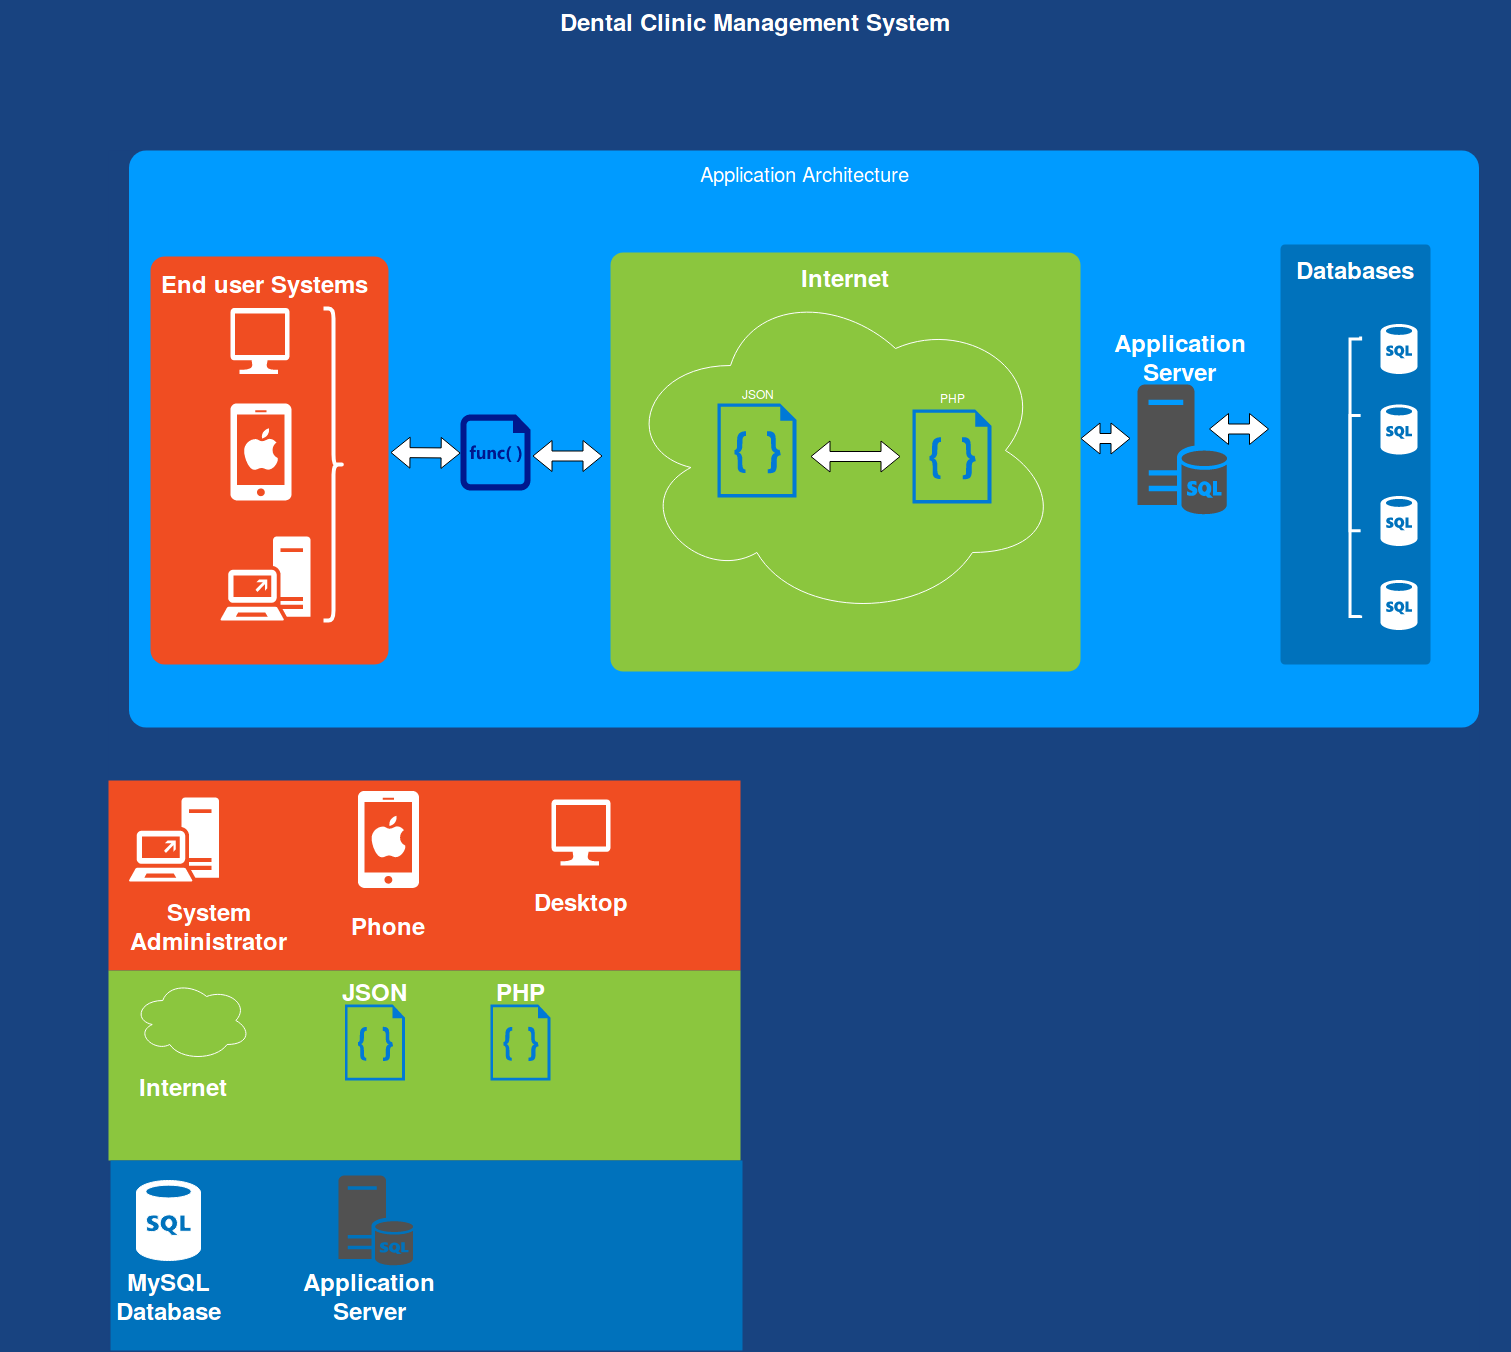
\includegraphics[width=\linewidth]{architecture.png}
    \caption{architecture}
    \end{figure}
    \newpage
    \subsubsection{Implemented Database Tables}
    \begin{figure}[h]
    \centering
    
    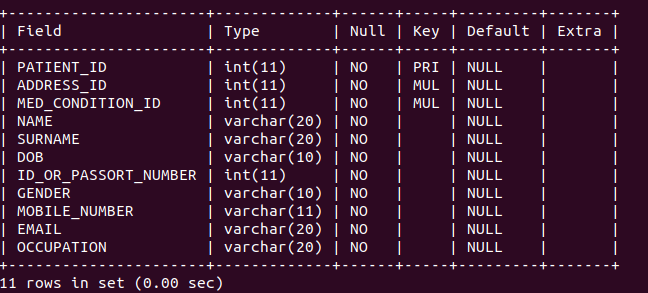
\includegraphics[width=\linewidth]{PATIENT_TABLE.png}
    \caption{Patient Table}
    \end{figure}
    \begin{figure}[h]
    \centering
    
    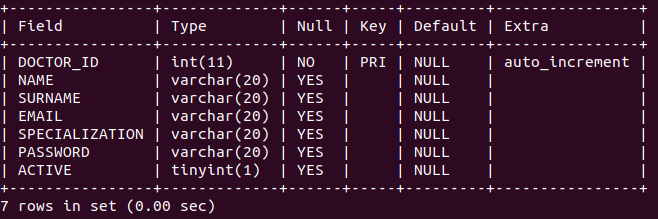
\includegraphics[width=\linewidth]{DOCTOR_TABLE.png}
    \caption{Doctor Table}
    \end{figure}
    
    \begin{figure}[h]
    \centering
    
    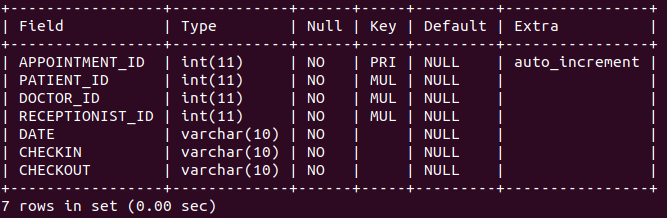
\includegraphics[width=\linewidth]{APPOINTMENT_TABLE.png}
    \caption{Doctor Table}
    \end{figure}
    
    \subsubsection{Entity Relationship Diagram}

    \begin{figure}[h]
    \centering
    
    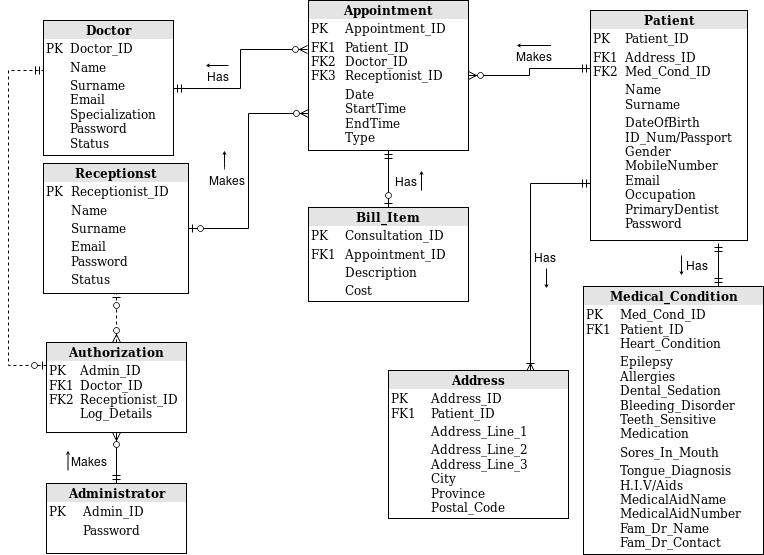
\includegraphics[width=\linewidth]{Dentist ERD.png}
    \caption{DCMS-ERD}
    \label{fig:ERD}
    \end{figure}
    
    \subsubsection{Software Tools}
    \begin{itemize}
    \item
     Database Server: Microsoft SQL Server
    \item
     Client: Any web browser
     \item
     Programming Language:Java
     \item
     Development Tools:Netbeans IDE 8.2
    \end{itemize}
    
    \subsubsection{Hardware Requirements}
The supported Operating Systems:
\begin{itemize}

\item
        \textbf{Microsoft Windows Vista SP1/Windows 7 Professional:}
        \begin{itemize}
        
            \item
            Processor: 800MHz Intel Pentium III or equivalent
            \item
            Memory: 512 MB
            \item
            Disk space: 750 MB of free disk space
            \end{itemize}
\item
        \textbf{Ubuntu 9.10:}
        \begin{itemize}
        \item
            Processor: 800MHz Intel Pentium III or equivalent
            \item
            Memory: 512 MB
            \item
            Disk space: 650 MB of free disk space
            \end{itemize}
        \item
        \textbf{Macintosh OS X 10.7 Intel:}
        \begin{itemize}
        
            \item
            Processor: Dual-Core Intel
            \item
            Memory: 2 GB
            \item
            Disk space: 650 MB of free disk space
            \end{itemize}
            \item
            \textbf{Smartphone Requirements:}
\begin{itemize}

\item
    Android running OS 4.0+
    \item
    iPhone running iOS 8+
    \item
    Windows Phone 8.1+
\end{itemize}
\end{itemize}
    \subsection{Product functions}
DCMS will enable patients to book or make appointment and the output will the be date and time in which it is inline with the Doctors schedule. System will
    also provide a clear schedule which allows patients to see
    which Doctor is available at a particular slot. Who ever
    will be using the system has to go through registration
    first if he/she is first time user or login by providing
    username and password to access the DCMS.The system allows patients to request their bill and the patient can view or print the through system.
\subsubsection{Use Case Diagram}

\begin{figure}[h]
    \centering
    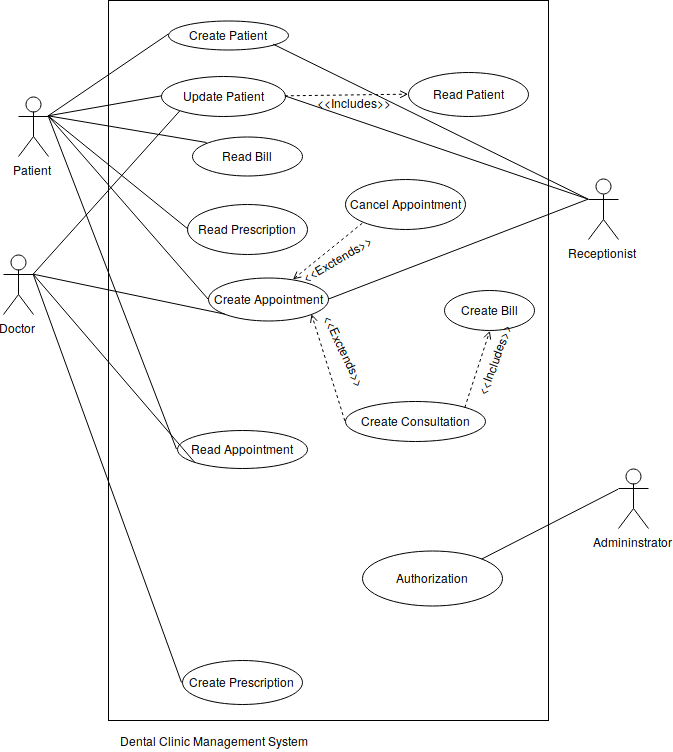
\includegraphics[scale = 0.5]{Use Case Diagram.png}
    \caption{DCMS-ERD}
    \label{fig:ERD}
    \end{figure}

    \subsection{Project Constraints}
    \begin{itemize}
    \item
    DCMS must run on any platform that supports Java.
    \item
    Data captured should be stored on a “cloud” database.
    \item
    The user needs to be connected to the internet.
    \end{itemize}
\section{Agile Approach:SCRUM}
\subsection{Scrum Roles}
\begin{itemize}
    \item
    Product owner - Represents the customer/users.  He Provides the specifications or requirements of the product, along with their priorities. This prioritized list of features is the product backlog.
    \item
    Scrum master - Enacts scrum values and practices. They Remove impediments, which are the obstacles that disrupt progress.
    \item
    Scrum team -perform analysis, design, program, test, document, and so forth
    \end{itemize}
  \subsection{Scrum Artifects}
  \subsubsection{User Stories}
  \textbf{Patient}
  \begin{itemize}
  \item
  As a patient, I want to be able to register on the system, so that I can have credentials to use to access the system
  \item
  As a patient, I want to be able to log in the system, so that I can access my portal on the system
  \item
  As a Patient, I want to be able to book an appointment, so that I can 				have a time reserved for me
  \item
  As a Patient, I want to be able to view my appointments, so that I can stay informed of the time and date.
  \item
  As a Patient, I want to be able cancel an appointment, so that I can change it's details without being charged a missed appintment fee.
  \item
  As a Patient, I want to be able view my bill, so that I can know all charges I have been charged.
  \end{itemize}
   \textbf{Dentist}
   \begin{itemize}
    \item
  As a Dentist, I want to be able to register on the system, so that I can have credentials to use to access the system
  \item
  As a Dentist, I want to be able to log in the system, so that I can access my portal on the system
  \item
  As a Dentist, I want to be able to view my schedule , so that I can stay informed.
  \item
  As a Dentist, I want to be able create a Consultation/Bill, so tha I can record all conducted procedures.
   \end{itemize}
   
\textbf{Receptionist}
   
    \begin{itemize}
  \item
  As a Receptionist, I want to be able to register on the system, so that I can have credentials to use to access the system
  \item
  As a Receptionist, I want to be able to log in the system, so that I can access my portal on the system
  \item
  As a Receptionist, I want to be able to book an appointment, so that I can 				have a time reserved for a requesting patient
  \item
   As a receptionist,  i want to be able to cancel an appointment, so that cancelled appointments are shown as such
   \end{itemize}
   \textbf{Administrator}:
   \begin{itemize}
   \item
   As an Administrator, I want to be able to authorize the creation of a new Doctor/Receptionist so that I can be able to ensure all relevent users are legitimate.
   \end{itemize}
  \subsubsection{Product Backlog}
  This is a list of prioritized features. The product backlog of DCMS is given below.
  
  \begin{figure}[h]
    \centering
    
    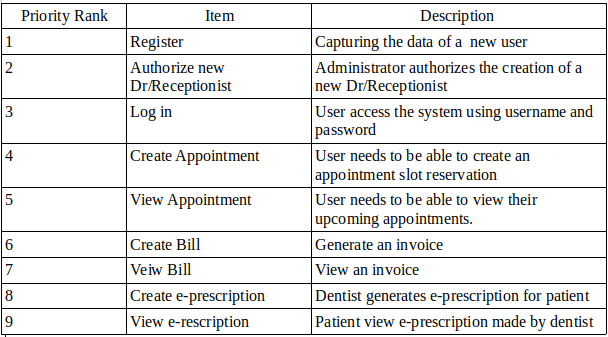
\includegraphics[width=\linewidth]{PriorityList.png}
    \caption{Priority List}
    \label{fig:ERD}
    \end{figure}
    
  \subsubsection{Sprint Backlog}
During the first sprint plan meeting, the product backlog was used to develop sprint backlogs.The first sprint comprises of 4 tasks/items. The tasks and their description are given below.
\begin{figure}[h]
    \centering
    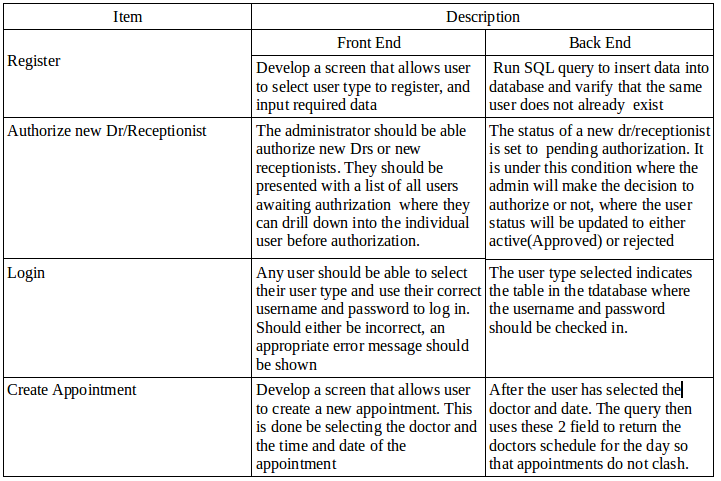
\includegraphics[width=\linewidth]{final.png}
    \caption{Sprint 1}
    \label{fig:ERD}
    \end{figure}

\newpage
Each task was estimated to take at most 10 hrs.The first sprints ran for 5 days.Daily scrum meetings were conducted to check the progress of each team member and to unblock any impediments.At the end of each sprint,  sprint review meetings were conducted to test and demostrate the functionality of the product.A sprint burn down diagram which shows the progress of the first sprint is given below 
\begin{figure}[h]
    \centering
    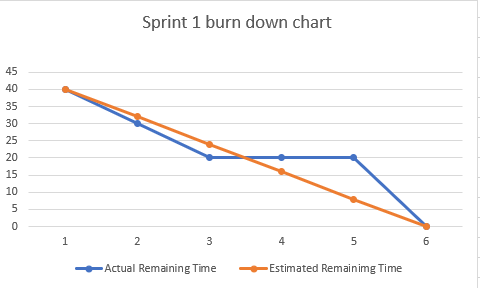
\includegraphics[width=\linewidth]{sprint1.PNG}
    \caption{Sprint 1 burndown diagram}
    \label{fig:ERD}
\end{figure}
    \newpage
During the second sprint plan meeting, the product backlog was used to develop sprint backlogs.The second sprint comprises of  6 tasks/items. The tasks and their description are given below.

\newpage
\begin{figure}[h]
    \centering
    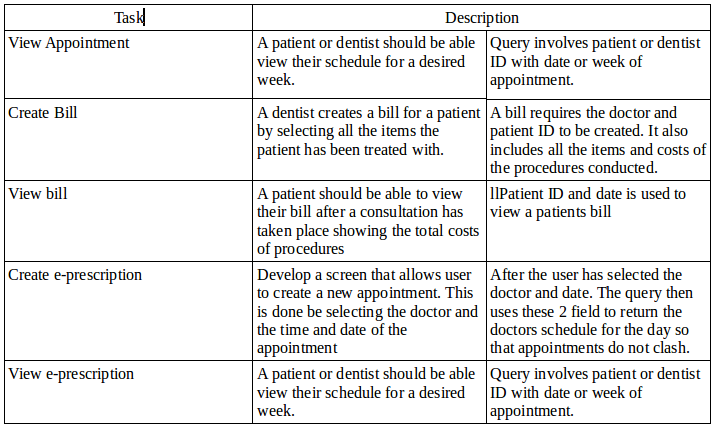
\includegraphics[width=\linewidth]{sprint2.PNG}
    \caption{Sprint 2}
    \label{fig:ERD}
\end{figure}

A second sprint of 5 tasks was formed from the product backlog.Each tasks was estimated to take at most 10 hrs and the sprint ran for 9 days.The tasks and their description are given below.A sprint burn down diagram which shows the progress of the second sprint is given below 
\begin{figure}[h]
    \centering
    
    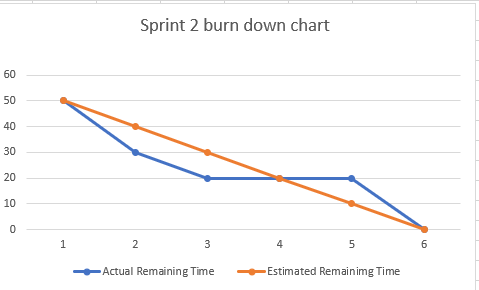
\includegraphics[width=\linewidth]{sprint3.PNG}
    \caption{Burn down diagram}
    \label{fig:ERD}
    \end{figure}
    \newpage
\section{Module Descriptions and Demonstrations} 
\subsection{Sceenshots}
\section{System development review method} 
\subsection{Sprint retrospective}
What went right 
\begin{itemize}
\item 


\end{itemize}
What went wrong

\begin{itemize}
\item Many tasks were underestimated
\item Scrum meetings were not effective, we did not hold  

\end{itemize}
What should we do differently
\begin{itemize}
\item k
\end{itemize}













\section{System Testing}
\subsection{Unit Tests}
Unit testing also called component testing was performed on standalone modules to check whether they were developed correctly. The following standalone modules were tested
\begin{itemize}
\item \textbf{Login}
\begin{figure}[h]
    \centering
    
    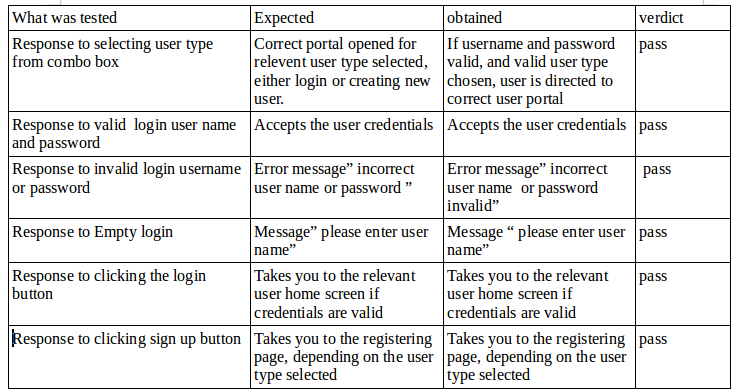
\includegraphics[width=\linewidth]{Logins.png}
    \caption{login testing}
    \label{fig:ERD}
    \end{figure}
\newpage
\item \textbf{Register}
\begin{figure}[h]
    \centering
    
    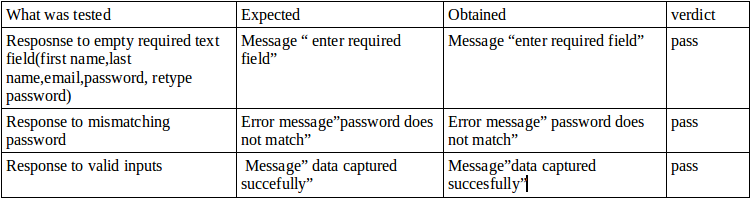
\includegraphics[width=\linewidth]{register.png}
    \caption{Register testing}
    \label{fig:ERD}
    \end{figure}

\end{itemize}

 \end{document}


